\begin{definition}
   Sea $\boldsymbol{\Sigma}:D\subseteq\Rn{2} \to\Rn{3}$ una parametrizaci\'on continua e  inyectiva de una superficie $S$. Si $ \partial D$ es la curva cerrada, simple,  frontera del conjunto $D$,  se define el \textbf{borde} o \textbf{frontera} de $S$, y se lo nota $\partial S$, a la curva cerrada simple en $\Rn{3}$ tal que 
    \[
        \partial S=\boldsymbol{\Sigma}(\partial D).
    \]
\end{definition}

\begin{obs} 
    Si $\partial D$ est\'a orientada de manera antihoraria, entonces $\boldsymbol{\Sigma}$ \textbf{induce} una orientaci\'on sobre $\partial S$. Adem\'as $\boldsymbol{\Sigma}$ \textbf{induce} una orientaci\'on sobre $S$.
\end{obs}

\textcolor{red}{Mano derecha. Explicacion e ilustracion}


\begin{definition} \textcolor{red}{mandar a topologia y referenciar}
    Sea $D$ un conjunto conexo (en $\Rn{2}$ o en $\Rn{3}$).  $D$ se llama \textbf{simplemente conexo}  si toda curva cerrada y  simple  $C\subset D$  es el borde de un conjunto $\hat{D}$ tal que $\hat{D} \subset  D.$
\end{definition}

\begin{theorem}
    \textbf{Teorema de Green}. Sea $D\subset \Rn{2}$ un conjunto simplemente conexo y sea   la curva simple y cerrada  $\partial D$ su frontera. Si  $\mathbf{F}:D\to\Rn{2}$  es continuo y de clase $\mathcal{C}^1$, entonces
    \[
        \oint_{\partial D^{+}} \mathbf{F}\cdot d\mathbf{s} = \iint_D \grad\times\mathbf{F}\cdot d\mathbf{A}.
    \]
\end{theorem}

\begin{obs}  \textcolor{red}{Notacion: dar}
   \[
        \int_{\partial D}P\:dx+Q\:dy=.
\]
\end{obs}




\begin{obs}
    \textbf{Extensi\'on de Green.} El teorema de Green es aplicable a regiones a\'un m\'as generales que simplemente conexas. De hecho, a cualquier regi\'on en $\Rn{2}$ cuya frontera se pueda descomponer en un n\'umero finito de curvas cerradas simples orientadas se le puede aplicar el teorema de Green. La idea es ``recorrer" dicha frontera pasando por todas las curvas que la confroman. 
    
    Por ejemplo, sea $D=D_1\cup D_2\cup D_3$ una regi\'on en $\Rn{2}$ no simplemente conexa, como muestra la figura a continuaci\'on.
    
    \begin{center}
    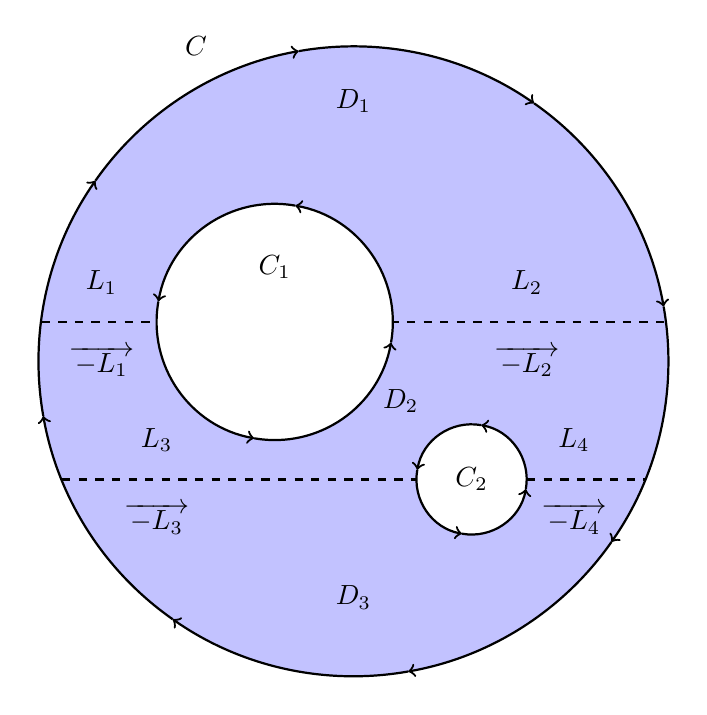
\begin{tikzpicture}
        % Define the exterior boundary with clockwise arrows
        \fill[blue!60!white!40] (0,0) circle (4);
        \foreach \angle in {315, 270, 225, 180, 135, 90, 45, 0} {
            \draw[thick, ->] ({4*cos(\angle+10)}, {4*sin(\angle+10)}) 
                arc[start angle=\angle+10, end angle=\angle-45+10, radius=4];
        }
        
        \draw[thick, dashed] (-3.96, 0.5) -- (3.96, 0.5);
        \draw[thick, dashed] (-3.7, -1.5) -- (3.7, -1.5);
        
        % Inner circle 1 with counterclockwise arrows
        \fill[white] (-1,0.5) circle (1.5);
        \foreach \angle in {0, 90, 180, 270} {
            \draw[thick, ->] ({-1+1.5*cos(\angle+80)}, {0.5+1.5*sin(\angle+80)}) 
            arc[start angle=\angle+80, end angle=\angle+170, radius=1.5];
            }
            
            % Inner circle 2 with counterclockwise arrows
        \fill[white] (1.5,-1.5) circle (0.7);
        \foreach \angle in {0, 90, 180, 270} {
            \draw[thick, ->] ({1.5+0.7*cos(\angle+80)}, {-1.5+0.7*sin(\angle+80)}) 
                arc[start angle=\angle+80, end angle=\angle+170, radius=0.7];
                }

        % Labels for regions
        \node at (0,3.3) {$D_1$};
        \node at (0.6,-0.5) {$D_2$};
        \node at (0,-3) {$D_3$};
        \node at (-2, 4) {$C$};
        \node at (-1,1.2) {$C_1$};
        \node at (1.5,-1.5) {$C_2$};
        \node at (-3.2, 1) {$\underleftarrow{\;\;L_1\;\;}$};
        \node at (-3.2, 0) {$\overrightarrow{\:-L_1\:}$};
        \node at (2.2, 1) {$\underleftarrow{\;\;L_2\;\;}$};
        \node at (2.2, 0) {$\overrightarrow{\:-L_2\:}$};
        \node at (-2.5, -1) {$\underleftarrow{\;\;L_3\;\;}$};
        \node at (-2.5, -2) {$\overrightarrow{\:-L_3\:}$};
        \node at (2.8, -1) {$\underleftarrow{\;\;L_4\;\;}$};
        \node at (2.8, -2) {$\overrightarrow{\:-L_4\:}$};
    \end{tikzpicture}
    \end{center}

    El borde de $D$ es $\partial D=C\cup C_1\cup C_2$. Y las orientaciones est\'an definidas tal que $C$ sea horaria y $C_1$ y $C_2$ sean antihorarias. Para poder aplicar el teorema de Green, se puede pensar en subdividir la regi\'on $D$ en tres regiones que s\'i sean simplemente conexas $D_1$, $D_2$ y $D_3$. Dichas regiones las delimitan las curvas $L_1$, $L_2$, $L_3$ y $L_4$. Notar que al ``recorrer'' cada una de las regiones subdivididas, las integrales sobre $L_1$, $L_2$, $L_3$ y $L_4$ se ``cancelan'' entre las regiones lim\'itrofes ya que poseen orientación opuesta. 
    
    Por lo tanto, si $\mathbf{F}$ es un campo vectorial definido en $D$, aplicando el teorema de Green.
    \begin{align*}
        \oint_{\partial D} \mathbf{F}\cdot d\mathbf{s}=&\oint_{C}\mathbf{F}\cdot d\mathbf{s}+\oint_{C_1}\mathbf{F}\cdot d\mathbf{s}+\oint_{C_2}\mathbf{F}\cdot d\mathbf{s}\\[.2cm]
        =&\oint_{\partial D_1}\mathbf{F}\cdot d\mathbf{s}+\oint_{\partial D_2}\mathbf{F}\cdot d\mathbf{s}+\oint_{\partial D_1}\mathbf{F}\cdot d\mathbf{s}\\[.2cm]
        =&\iint_{ D_1}\grad\times\mathbf{F}\cdot d\mathbf{A}+\iint_{ D_2}\grad\times\mathbf{F}\cdot d\mathbf{A}+\iint_{ D_1}\grad\times\mathbf{F}\cdot d\mathbf{A}\\[.2cm]
        =&\iint_D \grad\times\mathbf{F}\cdot d\mathbf{A}
    \end{align*}
    Lo que significa que el teorema de Green se puede aplicar a regiones no simplemente conexas.
\end{obs}

\begin{theorem}
\textbf{Teorema de la divergencia en el plano}. Sea $D\subset\Rn{2}$ una regi\'on donde valga el teorema de Green y sea $\partial D$ su frontera. Denotaremos por $\mathbf{n}$ el versor unitario normal a $\partial D$.  Si $\boldsymbol{\sigma}:[a,b]\to\Rn{2},\;\boldsymbol{\sigma}(t)=(x(t),y(t))$ es una parametrizaci\'on que recorre a $\partial D$ de manera positiva,  entonces  $\mathbf{n}$ est\'a dado por 
\[
    \mathbf{n}=\frac{(y'(t),-x'(t))}{\sqrt{[x'(t)]^2+[y'(t)]^2}}.
\]
Si $\mathbf{F}:  D\to \Rn{2}$ es un campo vectorial continuo y de clase $\mathcal{C}^1(\interior{D})$,  entonces
\[
    \int_{\partial D}\mathbf{F}\cdot\mathbf{n}\:ds=\iint_D\grad\cdot\mathbf{F}\:dA.
\]
\end{theorem}


\textcolor{red}{explicar:  son las inducidas por $\boldsymbol{\Sigma}$. Se puede referenciar a la regla de la mano derecha}

\begin{theorem}
\textbf{Teorema de Stokes}. Sea $\boldsymbol{\Sigma}:D\subset\Rn{2} \to S\subset\Rn{3}$    una parametrizaci\'on de una superficie $S$.   Si $\mathbf{F}:  A\subset \Rn{3}\to \Rn{3}$ es un campo vectorial continuo, de clase  $\mathcal{C}^1(\interior{A})$ tal que  $S \subset A$, entonces
\[
    \oint_{\partial S}\mathbf{F}\cdot d\mathbf{s}=\iint_S\grad\times\mathbf{F}\cdot d\mathbf{A}, 
\]  donde las orientaciones tanto de  $S$ como de $\partial S$ son las inducidas por $\boldsymbol{\Sigma}$ sobre ellas.

\end{theorem}

\begin{theorem}
\textbf{Teorema de la divergencia o de Gauss}. Sea $S\subset\Rn{3}$ una superficie que encierra un volumen $\Omega$ ( $S=\partial \Omega$ ) orientada de manera exterior.  Si $\mathbf{F}:A \subset \Rn{3} \to\Rn{3}$ es  un campo vectorial continuo y de clase $\mathcal{C}^1(\interior{A})$ tal que $\Omega \subset \interior{A}$, entonces
\[
    \oiint_{\partial \Omega}\mathbf{F}\cdot d\mathbf{S}=\iiint_{\Omega}\grad\cdot\mathbf{F}\:dV.
\]
\end{theorem}